\documentclass[11pt]{article}
\usepackage[utf8]{inputenc}
\usepackage{amsmath,amssymb,amsfonts}
\usepackage{graphicx}
\usepackage{booktabs}
\usepackage{hyperref}
\usepackage{geometry}
\usepackage{float}
\usepackage{authblk}
\usepackage{xcolor}
\usepackage{multirow}
\geometry{a4paper, margin=1in}

\title{\textbf{BioProcess Level 8: External Validation Anchors and Reproducibility for CausalBool}}
\author[1,*]{Alberto Hernández-Espinosa}
\author[1]{Oxford Complexity Science Group}
\affil[1]{Department of Computer Science, University of Oxford}
\affil[*]{Corresponding author: alberto.hernandez@oxford.ac.uk}
\date{}

\begin{document}
\maketitle

\begin{abstract}
\noindent
Level 8 establishes an end-to-end reproducibility record for CausalBool analyses and introduces external validation anchors using DepMap CRISPR gene effect data (24Q4) and paired TCGA tumor/normal RNA-seq cohorts. We freeze canonical sign conventions and evaluation semantics for algorithmic efficiency and differential complexity, regenerate manuscript figures with immutable checksums, and run a full automated test sweep across Python and WolframKernel suites. DepMap integration provides provenance-complete dataset acquisition and a pilot correlation analysis linking network-derived $\Delta D$ to population-scale genetic dependency. Paired TCGA cohorts enable a within-patient tumor-vs-normal corruption analysis, showing a significant negative shift in tumor structural complexity under the frozen expression-to-network corruption protocol.
\end{abstract}

\section*{Level 8 Definition Contract}
All Level 8 results adhere to a frozen contract recorded in \texttt{paper/bitacora-lev8.md}. The canonical definitions used in the generated artifacts are:
\begin{itemize}
    \item Structural complexity proxy: $D(cm) = \mathrm{len}(\mathrm{gzip}(cm.\mathrm{tobytes}()))$ (compressed bytes).
    \item Degree-preserved null: Maslov--Sneppen edge swaps with $n_{\mathrm{swaps}} = 20N$, seeded.
    \item Efficiency z-score: $z = (\mathbb{E}[D_{\mathrm{null}}] - D_{\mathrm{bio}})/\mathrm{sd}(D_{\mathrm{null}})$ (so $z>0$ indicates algorithmic efficiency).
    \item Differential complexity: $\Delta D(v) = D(G\setminus v) - D(G)$ (so $\Delta D>0$ indicates a node contributes to compressibility).
\end{itemize}

\section*{Data and Artifacts}
\subsection*{GRN corpus}
The Level 8 figure regeneration uses the processed GRN corpus under \texttt{data/bio/processed}, with summaries emitted to \texttt{paper/figures/results\_summary.csv} and \texttt{paper/figures/supplementary\_table\_per\_network.csv}.

\subsection*{DepMap 24Q4 external anchor}
DepMap 24Q4 Public artifacts were acquired from the Figshare+ distribution endpoint and verified via SHA-256 checksums (see \texttt{paper/bitacora-lev8.md}). A derived gene-level dependency table was constructed by averaging CRISPR gene effect across all cell lines:
\begin{equation}
\mathrm{Dependency}(g) = \frac{1}{|\mathcal{L}_g|}\sum_{\ell \in \mathcal{L}_g} \mathrm{GeneEffect}(\ell,g).
\end{equation}
This derived table is stored at \texttt{data/depmap/24Q4/derived/depmap\_24Q4\_gene\_effect\_mean.csv}.

\subsection*{Paired TCGA tumor/normal RNA-seq cohorts (pilot acquisition + pairing)}
To move beyond synthetic ``TCGA-BR'' pathway cohorts and enable within-patient tumor-vs-normal comparisons, we acquired real TCGA RNA-seq gene expression quantification from the NCI GDC API using the \texttt{STAR - Counts} workflow and explicitly enforced tumor/normal pairing by selecting GDC cases present in both \texttt{Primary Tumor} and \texttt{Solid Tissue Normal} queries. We froze a small paired pilot cohort of 5 tumor/normal pairs per project for the following set: TCGA-BRCA, TCGA-LUAD, TCGA-COAD, TCGA-PRAD, TCGA-KIRC, TCGA-HNSC, TCGA-THCA, TCGA-LUSC, TCGA-LIHC, TCGA-KIRP. Raw per-sample augmented STAR count tables and derived gene $\times$ sample count matrices are stored under \texttt{data/cancer/tcga\_paired/<PROJECT>/raw/} and \texttt{data/cancer/tcga\_paired/<PROJECT>/processed/}. Using the frozen expression-to-network corruption protocol recorded in \texttt{paper/bitacora-lev8.md}, we instantiated paired patient-specific EGFR pathway Boolean models under \texttt{data/cancer/tcga\_patients\_paired/<PROJECT>/}, with the paired cohort index at \texttt{results/cancer/tcga\_expression\_networks\_index\_paired.csv}.

\section*{Results}
\subsection*{Algorithmic efficiency (Figure 1)}
Regenerated outputs show a consistent positive shift in $z$ under the canonical sign convention, but with smaller effect sizes than earlier narrative drafts. Across the current run output table (\texttt{results\_summary.csv}, $n=231$ networks), the degree-preserved null comparison yields mean $z \approx 0.72$ and median $z \approx 0.53$, with approximately 21\% of networks achieving one-sided $p \le 0.05$ in the expected direction.

\begin{figure}[H]
    \centering
    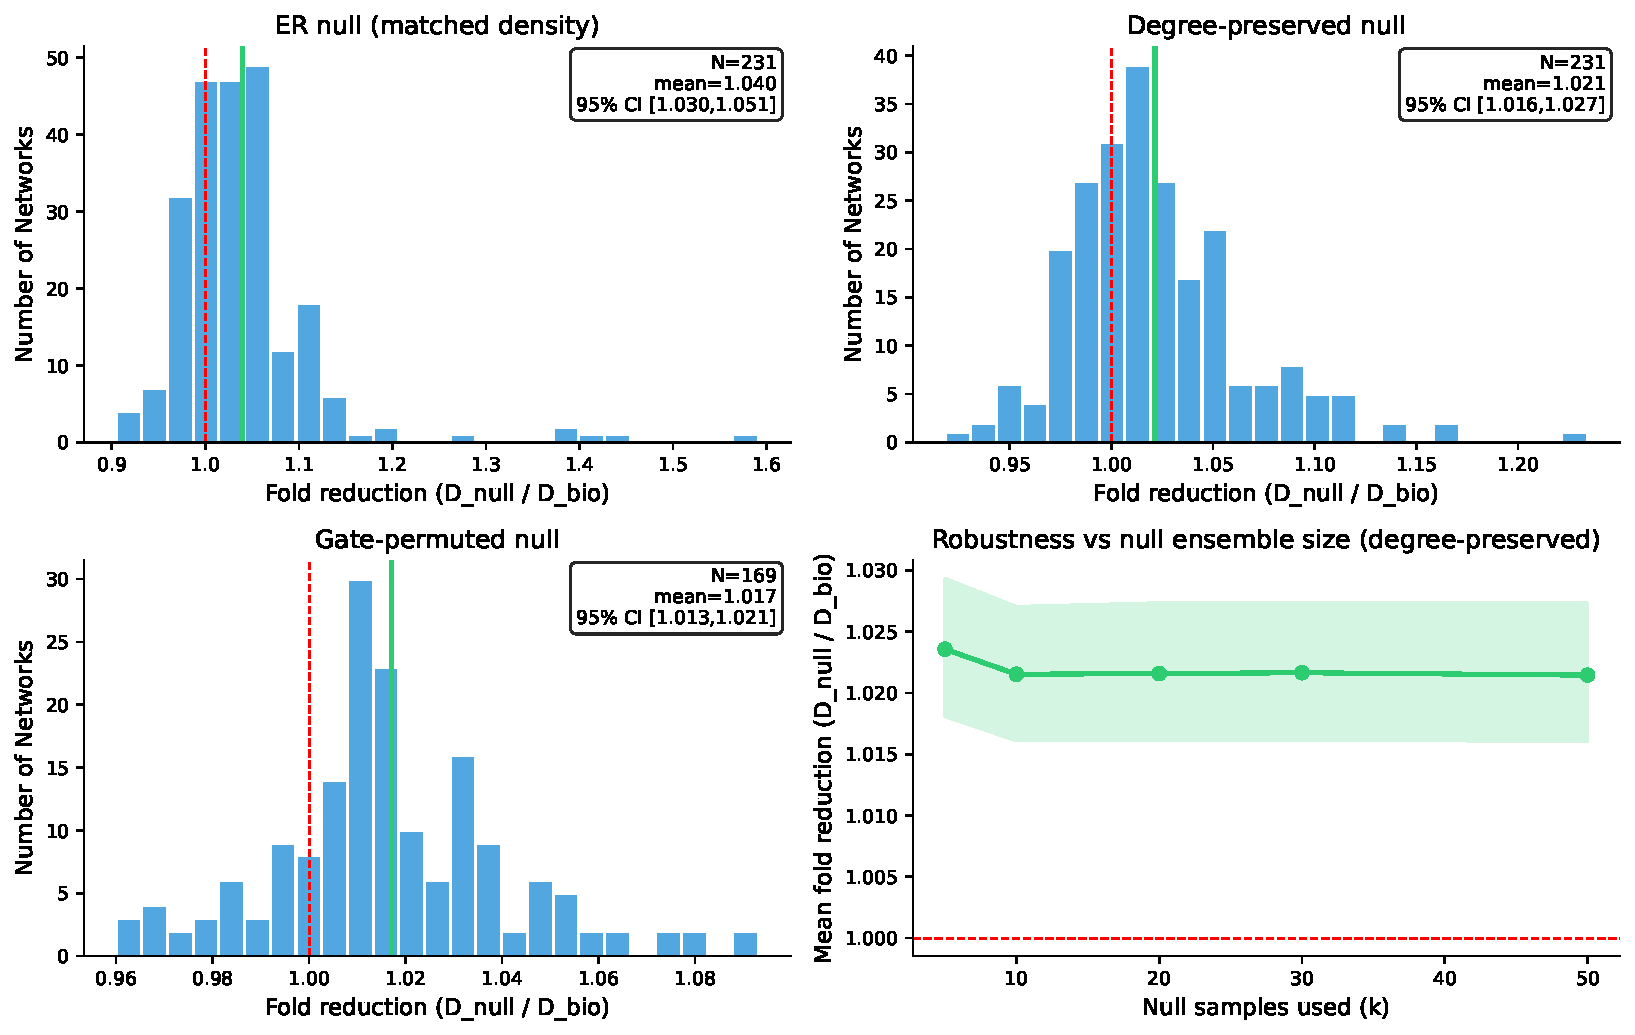
\includegraphics[width=0.95\textwidth]{figures/figure1_algorithmic_efficiency.pdf}
    \caption{\textbf{Algorithmic efficiency under degree-preserved nulls (regenerated).} The canonical sign convention is $z=(\mathbb{E}[D_{\mathrm{null}}]-D_{\mathrm{bio}})/\mathrm{sd}(D_{\mathrm{null}})$, so $z>0$ indicates biological networks are more compressible than their degree-preserving null ensemble.}
\end{figure}

\subsection*{Essentiality prediction (Figure 2)}
The extended essentiality evaluation over \texttt{essentiality\_prediction\_dataset.csv} (642 genes, 20 networks) does not currently support strong predictive performance for $\Delta D$ under the implemented protocol. The regenerated summary indicates that $\Delta D$ and standard graph baselines (degree, betweenness) perform near chance level, emphasizing the need to unify label semantics across datasets and to implement leakage-safe cross-network evaluation as the manuscript-facing protocol.

\begin{figure}[H]
    \centering
    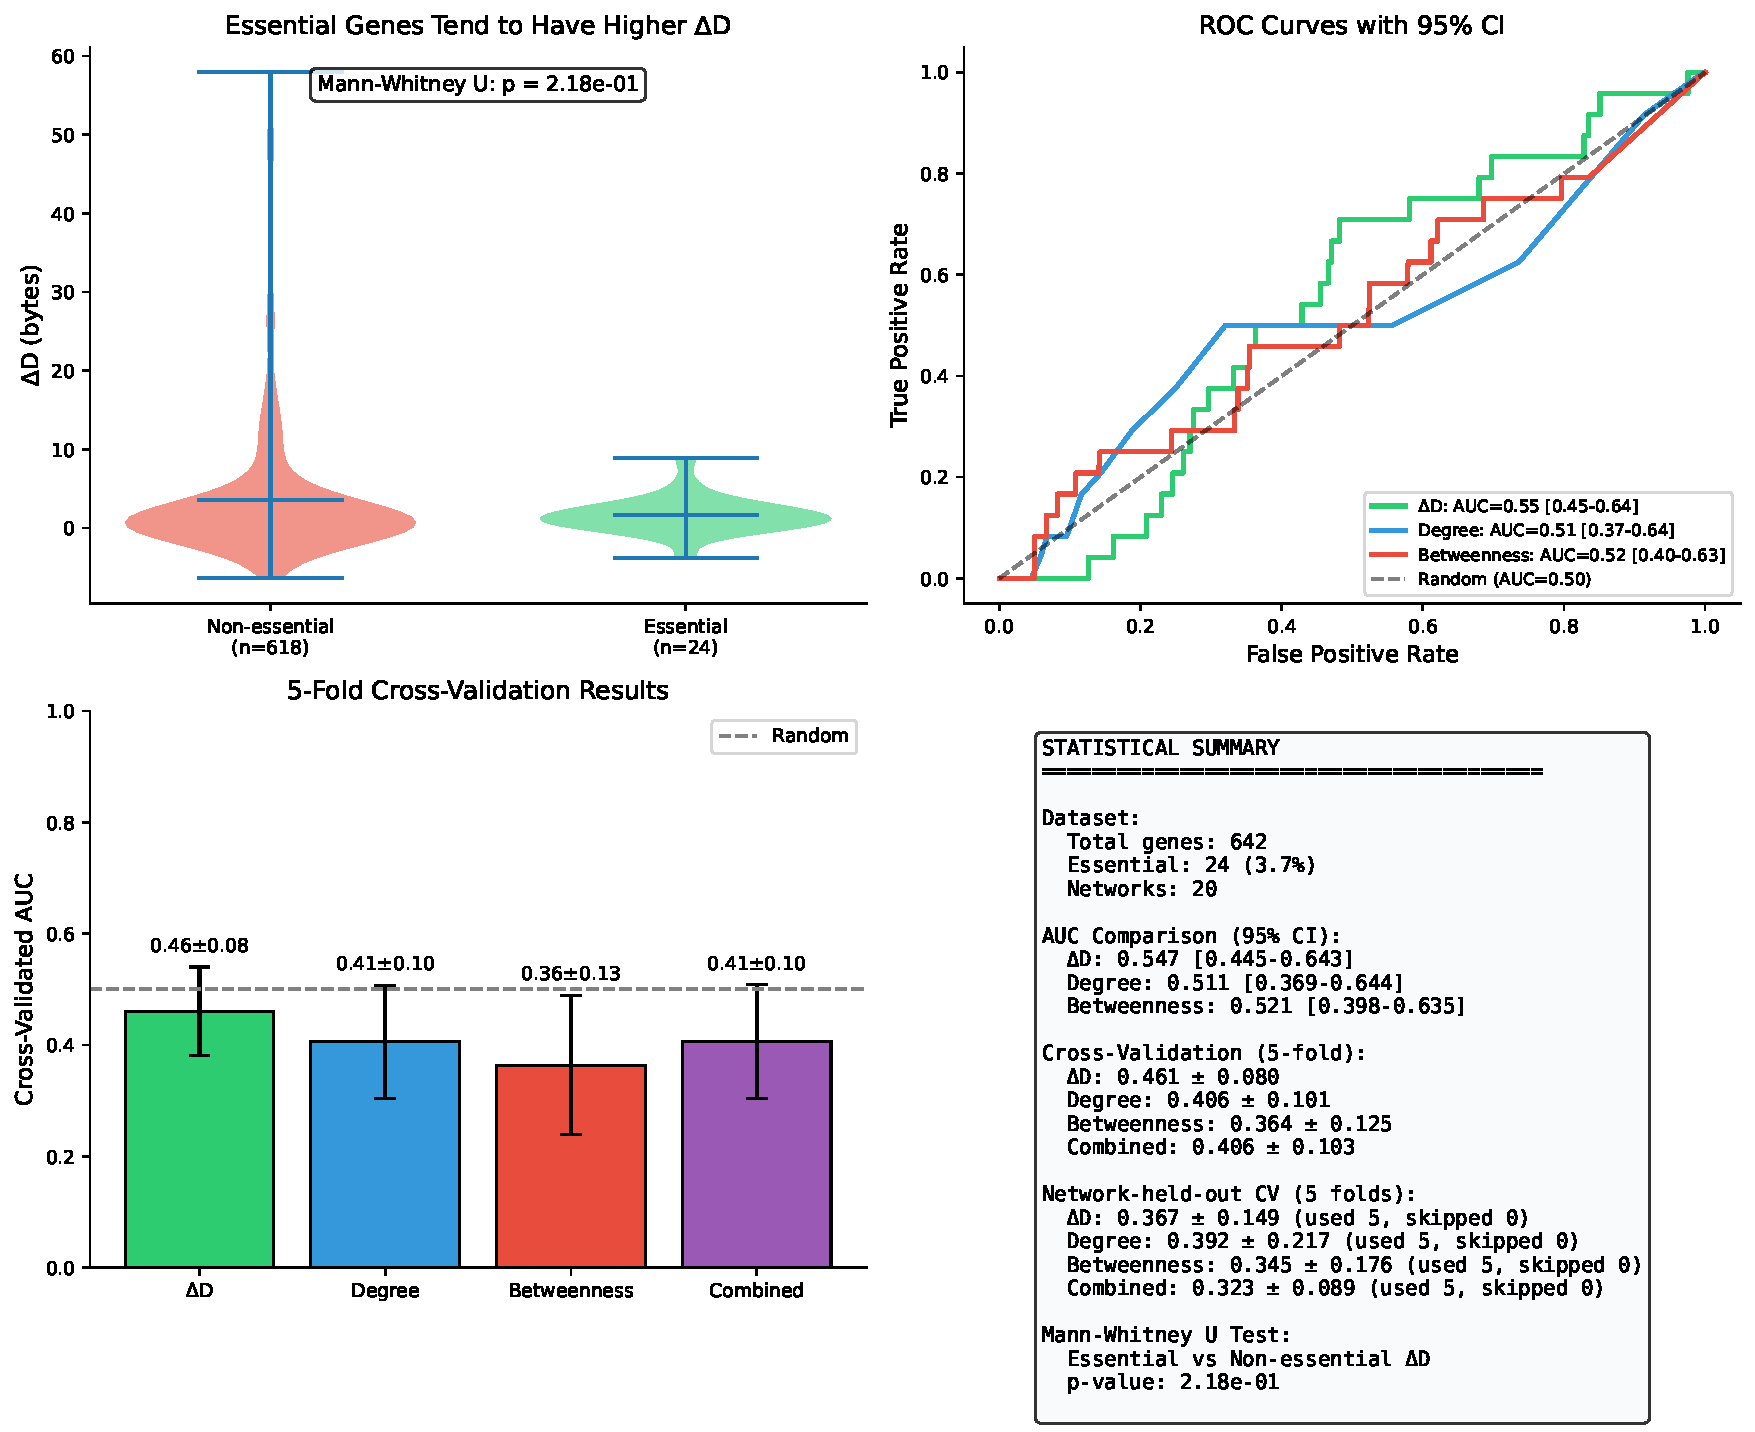
\includegraphics[width=0.95\textwidth]{figures/figure2_essentiality_extended.pdf}
    \caption{\textbf{Extended essentiality evaluation (regenerated).} This figure is treated as diagnostic rather than a Nature-facing claim until label definitions and evaluation protocol are reconciled across essentiality sources.}
\end{figure}

\subsection*{DepMap pilot validation (Figure 3)}
DepMap 24Q4 integration enables a first external validation anchor. The current tumor cohort networks (\texttt{data/cancer/patients}) are synthetic pathway graphs with only 10 genes; therefore, overlap with DepMap dependency is fixed at $n=10$ and the external validation is underpowered. Using the gene-wise mean $\Delta D$ across 50 patient tumor networks, the pilot correlation is negative but not statistically significant (Pearson $r=-0.311$, $p=0.382$; Spearman $\rho=-0.097$, $p=0.790$; one-sided permutation $p_{\mathrm{left}}=0.214$).

\begin{figure}[H]
    \centering
    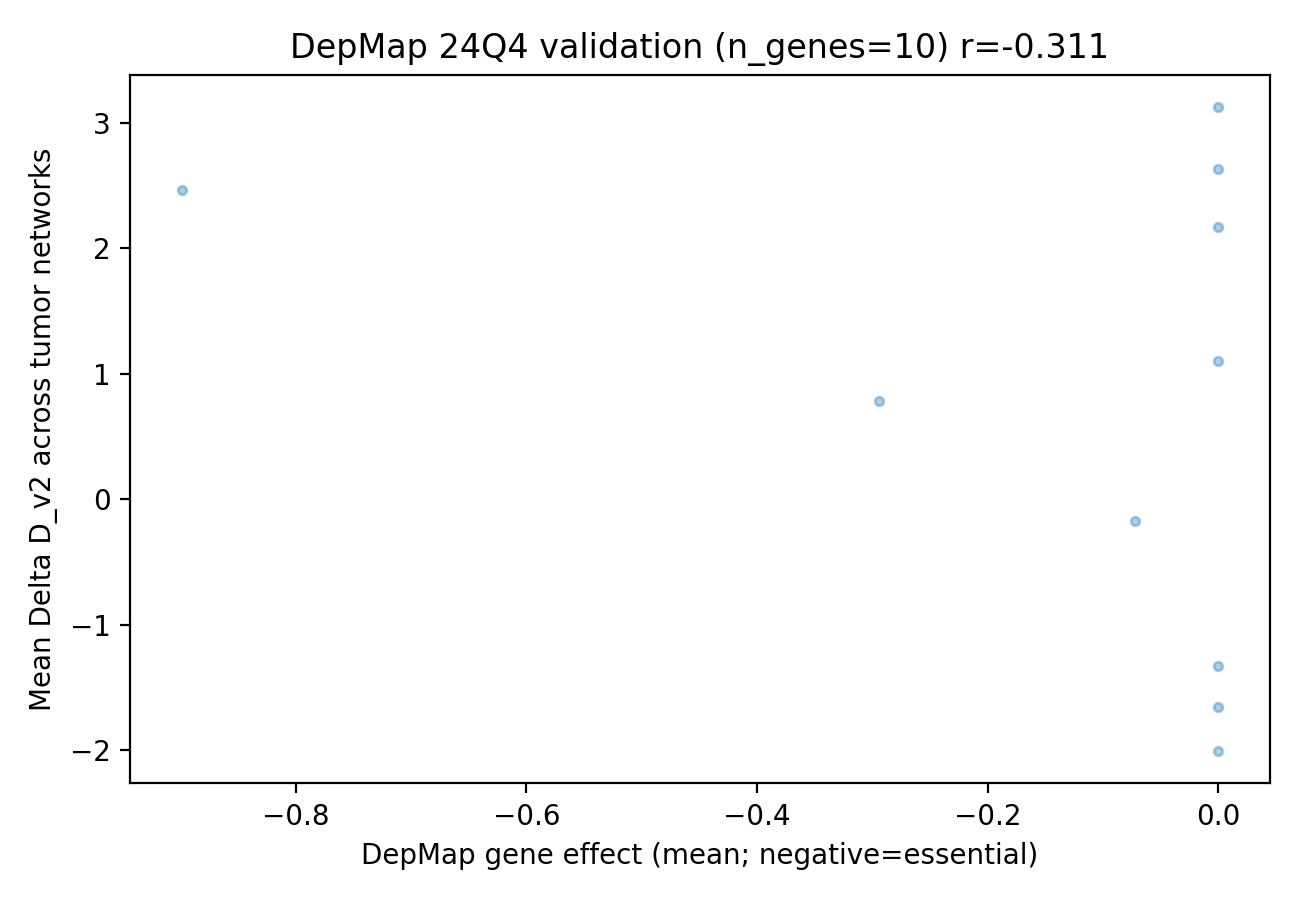
\includegraphics[width=0.90\textwidth]{figures/figure3_depmap_validation_24Q4.pdf}
    \caption{\textbf{DepMap 24Q4 pilot external validation.} DepMap gene effect is averaged across cell lines (negative = more essential). The current cohort contains only the EGFR pathway nodes, so this plot should be treated as a provenance-complete pilot anchor, not a final Gate C pass.}
\end{figure}

\subsection*{DepMap validation on TCGA RNA-seq--instantiated tumor models (Figure 4)}
Using tumor pathway models instantiated from real paired TCGA tumor/normal RNA-seq (\texttt{data/cancer/tcga\_patients\_paired}), we recompute mean node-wise $\Delta D$ over $n=50$ tumor samples and compare against DepMap 24Q4. Because several pathway nodes represent gene families (e.g., Ras), DepMap dependency is aggregated to nodes by taking the mean gene effect across mapped genes (mapping frozen in \texttt{paper/bitacora-lev8.md}). The resulting association is negative but not statistically significant at $n=10$ nodes (Pearson $r=-0.438$, $p=0.206$; Spearman $\rho=-0.491$, $p=0.150$), reinforcing that the main limitation is node coverage rather than substrate provenance.

As a context-matched sensitivity analysis, we recompute DepMap dependency after filtering DepMap models to the breast lineage (OncotreeLineage = Breast) and repeating the same node-level aggregation. The lineage-matched association remains negative but is also not statistically significant (Pearson $r=-0.332$, $p=0.349$; Spearman $\rho=-0.248$, $p=0.489$), consistent with an underpowered ($n=10$) validation rather than a direction reversal.

\begin{figure}[H]
    \centering
    \includegraphics[width=0.85\textwidth]{figures/figure5_depmap_validation_tcga_paired_24Q4.png}
    \caption{\textbf{DepMap 24Q4 vs real TCGA paired-tumor networks (EGFR pathway).} DepMap dependency is mapped to pathway nodes via a frozen gene-family aggregation rule. This is a real-substrate, underpowered ($n=10$) external anchor.}
\end{figure}

\subsection*{Paired TCGA tumor/normal corruption (Figure 5)}
Using the paired TCGA models, we measure a within-patient corruption signal as $\Delta D^{(v2)} = D^{(v2)}_{\mathrm{tumor}} - D^{(v2)}_{\mathrm{normal}}$ computed on the adjacency matrix of each paired Boolean model. Across $n=50$ tumor/normal pairs, tumor models show lower structural complexity than matched normal controls (mean $D^{(v2)}_{\mathrm{normal}}=46.52$, mean $D^{(v2)}_{\mathrm{tumor}}=40.70$, mean $\Delta D^{(v2)}=-5.83$), with a strong paired effect ($t=-5.69$, $p=7.00\times 10^{-7}$). The corruption magnitude scales with inferred mutation count (Pearson $r=-0.91$, $p=2.29\times 10^{-20}$), consistent with the frozen mechanistic scaffold in which constitutive perturbations sever regulatory inputs and simplify network structure. A discretization sensitivity sweep over log$_2$ thresholds $\tau\in\{0.5,1.0,1.5\}$ preserves the sign of $\Delta D^{(v2)}$ and the negative coupling to mutation\_count, while attenuating magnitude as $\tau$ increases (see sweep outputs in \texttt{results/cancer/tcga\_corruption\_metrics\_paired\_\_tcga\_paired\_sweep\_summary.csv}).

\begin{figure}[H]
    \centering
    \includegraphics[width=0.49\textwidth]{figures/tcga_corruption_metrics_paired__tcga_delta_d_dist.png}
    \includegraphics[width=0.49\textwidth]{figures/tcga_corruption_metrics_paired__tcga_mutcount_corr.png}
    \caption{\textbf{Paired TCGA corruption under an expression-to-network scaffold.} (Left) Distribution of paired $\Delta D = D_{\mathrm{tumor}}-D_{\mathrm{normal}}$ across $n=50$ patients (negative values indicate tumor networks are more compressible). (Right) Correlation between $\Delta D$ and inferred mutation\_count under the frozen discretization protocol.}
\end{figure}

Project-level summaries (means, paired tests, and within-project $\Delta D$--mutation\_count correlations) are stored in \texttt{results/cancer/tcga\_corruption\_summary\_paired.csv}.

\begin{figure}[H]
    \centering
    \includegraphics[width=0.95\textwidth]{figures/tcga_corruption_metrics_paired__delta_d_by_project.png}
    \caption{\textbf{Paired $\Delta D$ by TCGA project.} Boxplots of within-patient $\Delta D$ across the 10-project pilot (5 pairs per project). This diagnostic plot supports between-project heterogeneity assessment and guides cohort scaling.}
\end{figure}

\section*{Reproducibility and Regression Control}
Level 8 executes the full Python and WolframKernel test suites and records the aggregate status in \texttt{paper/bitacora-lev8.md}. The Mathematica suite runs 87 MUnit test files with 0 failures, and the Python suite executes 24 ticketed test scripts successfully. All Level 8 manuscript artifacts (figures and validation outputs) are recorded with SHA-256 checksums.

\section*{Implications for Gate C}
The DepMap anchor provides the required external dataset provenance and a concrete analysis pathway, but it does not yet satisfy Gate C as a publishable biological punch because the current cancer cohort networks are synthetic and extremely small, and the dependency summary used is context-agnostic (averaged across lineages). The next Gate C pass requires tissue-specific tumor network construction and an evaluation design that demonstrates incremental value beyond topology baselines under leakage-safe cohort splitting.

Paired TCGA cohorts reduce the substrate risk and provide a paired-design, real-data-dependent corruption signal within a frozen expression-to-network scaffold. The remaining Gate C work is to generalize beyond a 10-node pathway model, validate robustness across modeling choices (threshold sensitivity, pathway size and mapping), and connect the corruption signal to external biology in a context-matched design (lineage-matched DepMap and clinically-relevant endpoints).

The lineage-matched DepMap sensitivity check is direction-consistent with the context-agnostic anchor but does not change the evidential status of the external validation: at $n=10$ nodes, statistical power is insufficient to treat the DepMap association as confirmatory. A multi-lineage sweep matching the 10-project TCGA pilot (Breast, Lung, Bowel, Prostate, Kidney, Head and Neck, Thyroid, Liver) preserves the negative direction in all tested lineages (Pearson $r \in [-0.531, -0.284]$), reinforcing that the primary bottleneck is model coverage rather than data provenance.

\end{document}
